% AER-Article.tex for AEA last revised 22 June 2011
\documentclass[AER]{AEA}

% The mathtime package uses a Times font instead of Computer Modern.
% Uncomment the line below if you wish to use the mathtime package:
%\usepackage[cmbold]{mathtime}
% Note that miktex, by default, configures the mathtime package to use commercial fonts
% which you may not have. If you would like to use mathtime but you are seeing error
% messages about missing fonts (mtex.pfb, mtsy.pfb, or rmtmi.pfb) then please see
% the technical support document at http://www.aeaweb.org/templates/technical_support.pdf
% for instructions on fixing this problem.

% Note: you may use either harvard or natbib (but not both) to provide a wider
% variety of citation commands than latex supports natively. See below.

% Uncomment the next line to use the natbib package with bibtex
\usepackage{natbib}

% Uncomment the next line to use the harvard package with bibtex
%\usepackage[abbr]{harvard}

% This command determines the leading (vertical space between lines) in draft mode
% with 1.5 corresponding to "double" spacing.
\draftSpacing{1.5}

% Pandoc syntax highlighting
\usepackage{color}
\usepackage{fancyvrb}
\newcommand{\VerbBar}{|}
\newcommand{\VERB}{\Verb[commandchars=\\\{\}]}
\DefineVerbatimEnvironment{Highlighting}{Verbatim}{commandchars=\\\{\}}
% Add ',fontsize=\small' for more characters per line
\usepackage{framed}
\definecolor{shadecolor}{RGB}{248,248,248}
\newenvironment{Shaded}{\begin{snugshade}}{\end{snugshade}}
\newcommand{\AlertTok}[1]{\textcolor[rgb]{0.94,0.16,0.16}{#1}}
\newcommand{\AnnotationTok}[1]{\textcolor[rgb]{0.56,0.35,0.01}{\textbf{\textit{#1}}}}
\newcommand{\AttributeTok}[1]{\textcolor[rgb]{0.77,0.63,0.00}{#1}}
\newcommand{\BaseNTok}[1]{\textcolor[rgb]{0.00,0.00,0.81}{#1}}
\newcommand{\BuiltInTok}[1]{#1}
\newcommand{\CharTok}[1]{\textcolor[rgb]{0.31,0.60,0.02}{#1}}
\newcommand{\CommentTok}[1]{\textcolor[rgb]{0.56,0.35,0.01}{\textit{#1}}}
\newcommand{\CommentVarTok}[1]{\textcolor[rgb]{0.56,0.35,0.01}{\textbf{\textit{#1}}}}
\newcommand{\ConstantTok}[1]{\textcolor[rgb]{0.00,0.00,0.00}{#1}}
\newcommand{\ControlFlowTok}[1]{\textcolor[rgb]{0.13,0.29,0.53}{\textbf{#1}}}
\newcommand{\DataTypeTok}[1]{\textcolor[rgb]{0.13,0.29,0.53}{#1}}
\newcommand{\DecValTok}[1]{\textcolor[rgb]{0.00,0.00,0.81}{#1}}
\newcommand{\DocumentationTok}[1]{\textcolor[rgb]{0.56,0.35,0.01}{\textbf{\textit{#1}}}}
\newcommand{\ErrorTok}[1]{\textcolor[rgb]{0.64,0.00,0.00}{\textbf{#1}}}
\newcommand{\ExtensionTok}[1]{#1}
\newcommand{\FloatTok}[1]{\textcolor[rgb]{0.00,0.00,0.81}{#1}}
\newcommand{\FunctionTok}[1]{\textcolor[rgb]{0.00,0.00,0.00}{#1}}
\newcommand{\ImportTok}[1]{#1}
\newcommand{\InformationTok}[1]{\textcolor[rgb]{0.56,0.35,0.01}{\textbf{\textit{#1}}}}
\newcommand{\KeywordTok}[1]{\textcolor[rgb]{0.13,0.29,0.53}{\textbf{#1}}}
\newcommand{\NormalTok}[1]{#1}
\newcommand{\OperatorTok}[1]{\textcolor[rgb]{0.81,0.36,0.00}{\textbf{#1}}}
\newcommand{\OtherTok}[1]{\textcolor[rgb]{0.56,0.35,0.01}{#1}}
\newcommand{\PreprocessorTok}[1]{\textcolor[rgb]{0.56,0.35,0.01}{\textit{#1}}}
\newcommand{\RegionMarkerTok}[1]{#1}
\newcommand{\SpecialCharTok}[1]{\textcolor[rgb]{0.00,0.00,0.00}{#1}}
\newcommand{\SpecialStringTok}[1]{\textcolor[rgb]{0.31,0.60,0.02}{#1}}
\newcommand{\StringTok}[1]{\textcolor[rgb]{0.31,0.60,0.02}{#1}}
\newcommand{\VariableTok}[1]{\textcolor[rgb]{0.00,0.00,0.00}{#1}}
\newcommand{\VerbatimStringTok}[1]{\textcolor[rgb]{0.31,0.60,0.02}{#1}}
\newcommand{\WarningTok}[1]{\textcolor[rgb]{0.56,0.35,0.01}{\textbf{\textit{#1}}}}

% tightlist command for lists without linebreak
\providecommand{\tightlist}{%
  \setlength{\itemsep}{0pt}\setlength{\parskip}{0pt}}

% From pandoc table feature
\usepackage{longtable,booktabs,array}
\usepackage{calc} % for calculating minipage widths
% Correct order of tables after \paragraph or \subparagraph
\usepackage{etoolbox}
\makeatletter
\patchcmd\longtable{\par}{\if@noskipsec\mbox{}\fi\par}{}{}
\makeatother
% Allow footnotes in longtable head/foot
\IfFileExists{footnotehyper.sty}{\usepackage{footnotehyper}}{\usepackage{footnote}}
\makesavenoteenv{longtable}


\usepackage{graphicx}
\usepackage{booktabs}

\usepackage{hyperref}

\begin{document}


\title{Global \(CO_{2}\) Emissions in 1997}
\shortTitle{What Keeling missed all these years}
% \author{Author1 and Author2\thanks{Surname1: affiliation1, address1, email1.
% Surname2: affiliation2, address2, email2. Acknowledgements}}


\author{
  Carolyn Dunlap\\
  Ayda Nayeb Nazar\\
  Qian Qiao\\
  Hector Rincon\thanks{
  Dunlap: UC Berkeley, School of
Information, \href{mailto:cadunlap@ischool.berkeley.edu}{cadunlap@ischool.berkeley.edu}.
  Nayeb Nazar: UC Berkeley, School of
Information, \href{mailto:ayda@ischool.berkeley.edu}{ayda@ischool.berkeley.edu}.
  Qiao: UC Berkeley, School of
Information, \href{mailto:qianqiao@ischool.berkeley.edu}{qianqiao@ischool.berkeley.edu}.
  Rincon: UC Berkeley, School of
Information, \href{mailto:hector@ischool.berkeley.edu}{hector@ischool.berkeley.edu}.
  The authors would like to thank their instructors from MIDS 271.
}
}

\date{\today}
\pubMonth{03}
\pubYear{2023}
\pubVolume{0}
\pubIssue{0}
\JEL{}
\Keywords{Replication, Modern Science}

\begin{abstract}
This study analyzes the time series of atmospheric CO2 concentrations
from monitoring stations around the world that managed by the National
Oceanic and Atmospheric Administration (NOAA). Our goal is to develop a
model that accurately captures the trend and seasonality of CO2
concentrations over time, as well as any other relevant patterns or
anomalies. To accomplish this, various time series modeling techniques
are employed, including linear regression models and seasonal
autoregressive integrated moving average (ARIMA) models. The analysis
finds that a seasonal ARIMA model with a trend and seasonal difference
term provides the best fit to the CO2 time series data. This model
reveals a clear upward trend in CO2 concentrations over time, with
seasonal variations superimposed on top of this trend.
\end{abstract}


\maketitle

Climate change is one of the most pressing issues of our time. One of
the key contributors to climate change is the increase in atmospheric
carbon dioxide (CO2) levels. The Keeling Curve, created by Charles David
Keeling, shows the steady increase in atmospheric \(CO_{2}\) levels over
time. What the trend and seasonality lies in the atmospheric \(CO_{2}\)
changing? How can we use the trend and seasonality to to model the
future impacts of climate change? These are the core questions we want
to address.This analysis will help us to have a better understanding on
a changing climate and to develop strategies for mitigating its effects.

\hypertarget{background}{%
\section{Background}\label{background}}

\hypertarget{carbon-emissions}{%
\subsection{Carbon Emissions}\label{carbon-emissions}}

Carbon emissions are a major environmental concern because they
contribute to the Earth's rising temperature, which can cause a range of
negative impacts on the environment and human society. These impacts
include sea-level rise, more frequent and severe weather events, changes
in precipitation patterns, and the loss of biodiversity and ecosystem
services.

\hypertarget{measurement-and-data}{%
\section{Measurement and Data}\label{measurement-and-data}}

\hypertarget{measuring-atmospheric-carbon}{%
\subsection{Measuring Atmospheric
Carbon}\label{measuring-atmospheric-carbon}}

Our analysis will draw on atmospheric \(CO_{2}\) data. The data on
atmospheric carbon dioxide (CO2) levels is generated by the Global
Monitoring Laboratory (GML) of the National Oceanic and Atmospheric
Administration (NOAA), which operates a network of over 80 monitoring
stations around the world. The data is collected through continuous
measurements of atmospheric CO2 concentrations using highly precise
instruments, such as gas chromatographs and infrared analyzers. One of
the longest and most well-known records of this data is the Mauna Loa
CO2 record, which has been collected since 1958 at the Mauna Loa
Observatory in Hawaii.

These stations collect CO2 measurements on a continuous basis, with data
typically collected every 10 to 15 minutes and measure the concentration
of atmospheric CO2 using highly precise instruments, such as gas
chromatographs and infrared analyzers.

\hypertarget{historical-trends-in-atmospheric-carbon}{%
\subsection{Historical Trends in Atmospheric
Carbon}\label{historical-trends-in-atmospheric-carbon}}

Monthly Atmospheric carbon from 1959 to 1997 is plotted in plot below.
The time series plot shows an increasing trend from 1959 to 1997 and
there is a seasonal fluctuations every year.

The ACF plot shows a slow decline and while the PACF plot drops sharply
after the first lag and shows significance up to three lags, which
confirmed our observation from the time series plot that the \(CO_{2}\)
data has a trend pattern.

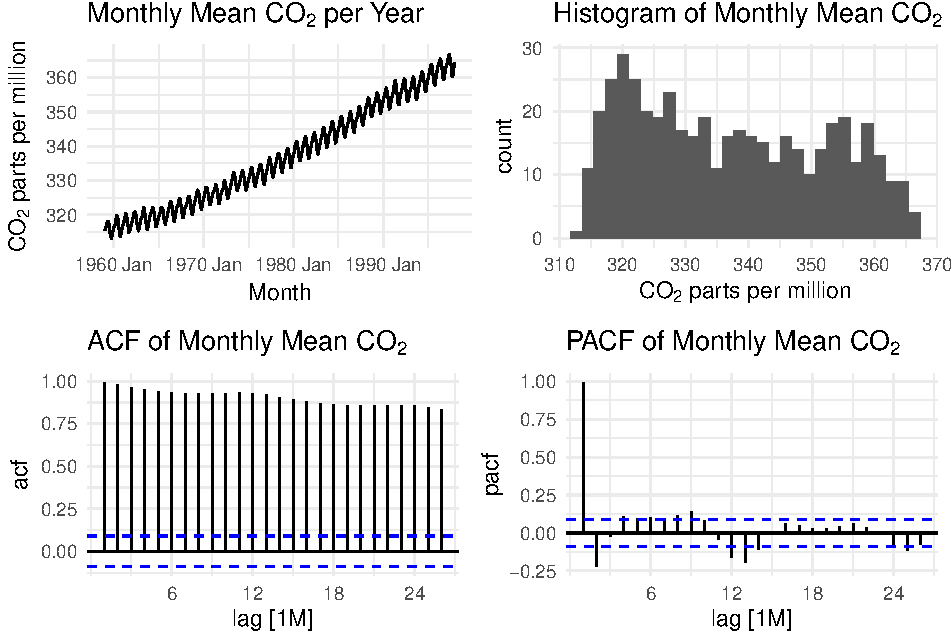
\includegraphics{co2_1997_Qian_files/figure-latex/EDA plots-1.pdf}

The seasonal plot displays a clear seasonality for each year. The
atmospheric \(CO_{2}\) level went to peak in April and May, and had the
yearly lowest \(CO_{2}\) pmm in September and October.

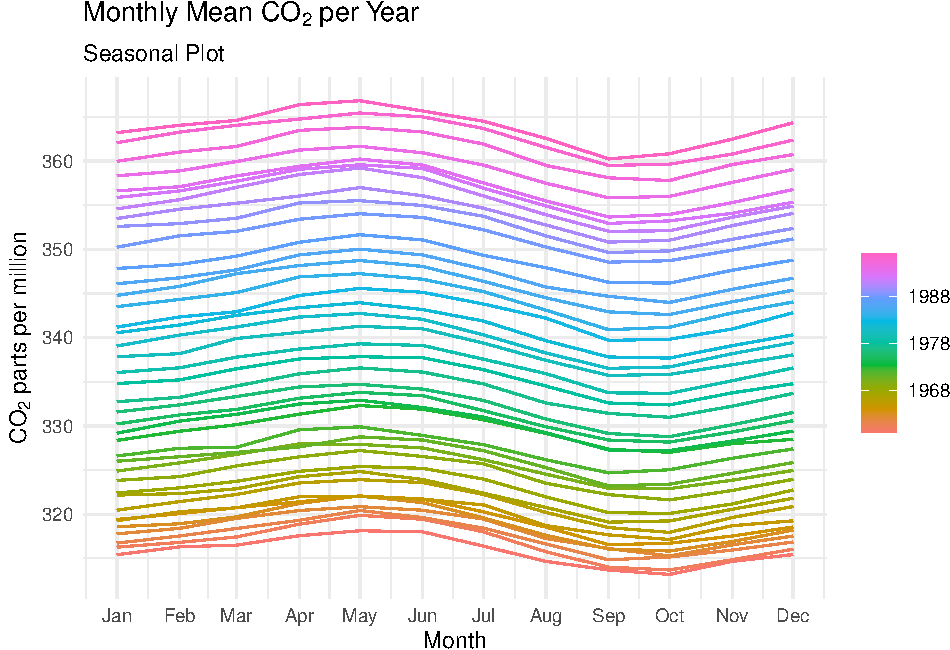
\includegraphics{co2_1997_Qian_files/figure-latex/seaonal grap-1.pdf}

Through the multiplicative composition plot, we observed a clear upward
trend in overall \(CO_2\) levels over time as well as seasonal patterns.

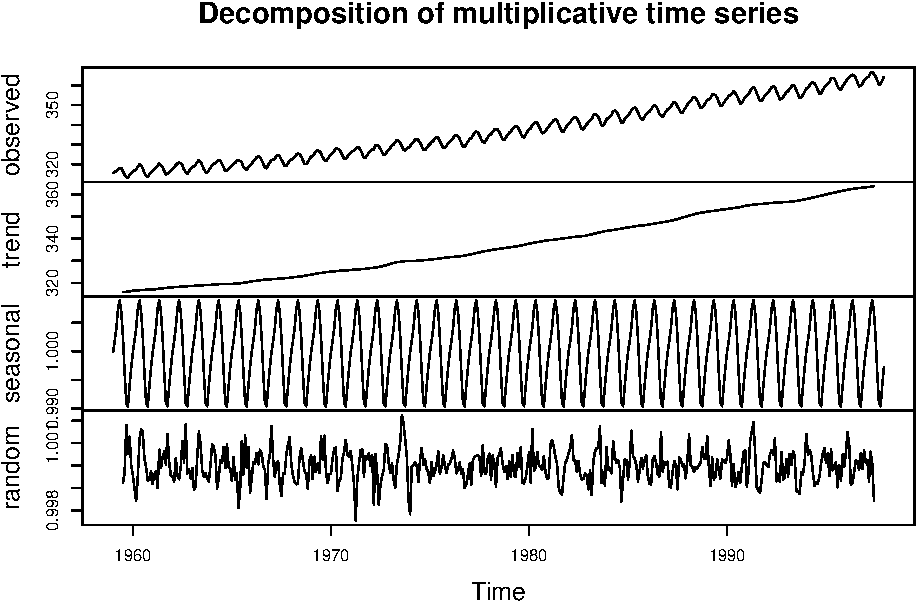
\includegraphics{co2_1997_Qian_files/figure-latex/decompose plot-1.pdf}

\hypertarget{models-and-forecasts}{%
\section{Models and Forecasts}\label{models-and-forecasts}}

To investigate the trend, seasonal, and irregular elements of the
\(CO_2\) data, we used linear regression and ARIMA method to model the
long-term increase in \(CO_2\) levels over time.

\hypertarget{linear-models}{%
\subsection{Linear Models}\label{linear-models}}

We begin by fitting the following simple linear model motivated by the
linear trend observed in the EDA:

\begin{equation}
\label{eq:one}
\text{CO}_{2} = \beta_0 + \beta t
\end{equation}

The model parameters are then estimated in the following way,

\begin{Shaded}
\begin{Highlighting}[]
\NormalTok{co2\_reg }\OtherTok{\textless{}{-}}\NormalTok{ ts\_co2 }\SpecialCharTok{\%\textgreater{}\%} 
    \FunctionTok{model}\NormalTok{(}\FunctionTok{TSLM}\NormalTok{(value }\SpecialCharTok{\textasciitilde{}} \FunctionTok{trend}\NormalTok{())) }\SpecialCharTok{\%\textgreater{}\%}
  \FunctionTok{report}\NormalTok{()}
\end{Highlighting}
\end{Shaded}

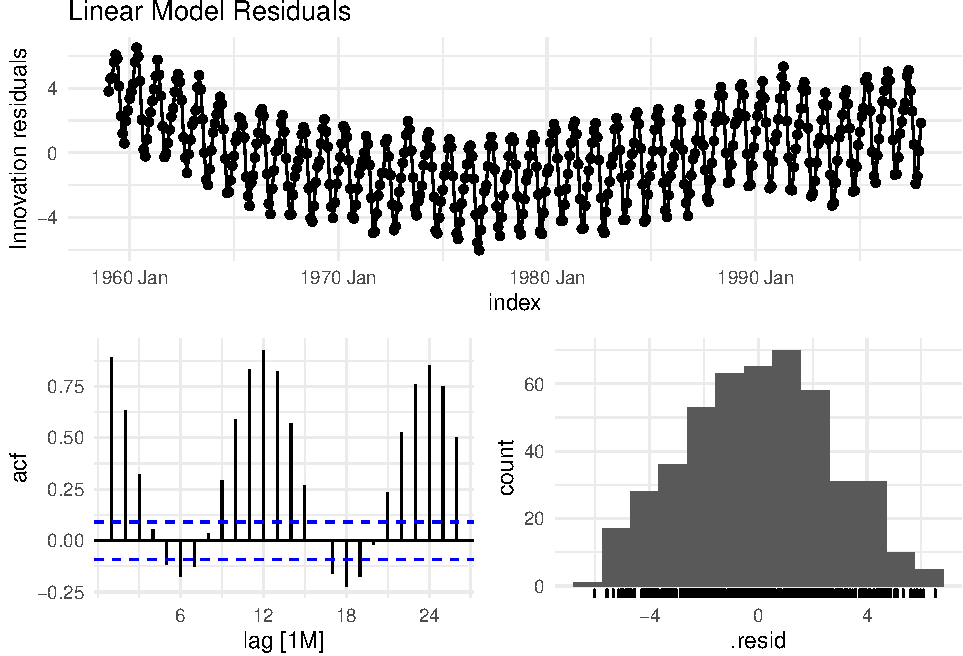
\includegraphics{co2_1997_Qian_files/figure-latex/linear model residuals-1.pdf}

Despite the strong linear trend observed in the time series plot, the
residuals of the simple linear model to not appear to be white noise as
showcases by the numerous significant lags and strong seasonal pattern
in the ACF plot. We can attempt to rectify this by incorporating
seasonal dummy variables into our model,

\begin{Shaded}
\begin{Highlighting}[]
\NormalTok{co2\_reg\_season }\OtherTok{\textless{}{-}}\NormalTok{ ts\_co2 }\SpecialCharTok{\%\textgreater{}\%} 
    \FunctionTok{model}\NormalTok{(}\FunctionTok{TSLM}\NormalTok{(value }\SpecialCharTok{\textasciitilde{}} \FunctionTok{trend}\NormalTok{() }\SpecialCharTok{+} \FunctionTok{season}\NormalTok{())) }\SpecialCharTok{\%\textgreater{}\%}
  \FunctionTok{report}\NormalTok{()}
\end{Highlighting}
\end{Shaded}

\begin{verbatim}
## Series: value 
## Model: TSLM 
## 
## Residuals:
##    Min     1Q Median     3Q    Max 
##  -2.77  -1.28  -0.41   1.26   4.34 
## 
## Coefficients:
##                 Estimate Std. Error t value Pr(>|t|)    
## (Intercept)    311.42208    0.29171 1067.57  < 2e-16 ***
## trend()          0.10921    0.00056  195.00  < 2e-16 ***
## season()year2    0.66336    0.37054    1.79  0.07408 .  
## season()year3    1.40543    0.37054    3.79  0.00017 ***
## season()year4    2.53597    0.37054    6.84  2.5e-11 ***
## season()year5    3.01445    0.37054    8.14  4.0e-15 ***
## season()year6    2.35140    0.37055    6.35  5.4e-10 ***
## season()year7    0.83039    0.37055    2.24  0.02551 *  
## season()year8   -1.23728    0.37056   -3.34  0.00091 ***
## season()year9   -3.06162    0.37056   -8.26  1.6e-15 ***
## season()year10  -3.24441    0.37057   -8.76  < 2e-16 ***
## season()year11  -2.05490    0.37058   -5.55  5.0e-08 ***
## season()year12  -0.93744    0.37059   -2.53  0.01176 *  
## ---
## Signif. codes:  0 '***' 0.001 '**' 0.01 '*' 0.05 '.' 0.1 ' ' 1
## 
## Residual standard error: 1.64 on 455 degrees of freedom
## Multiple R-squared: 0.988,   Adjusted R-squared: 0.988
## F-statistic: 3.22e+03 on 12 and 455 DF, p-value: <2e-16
\end{verbatim}

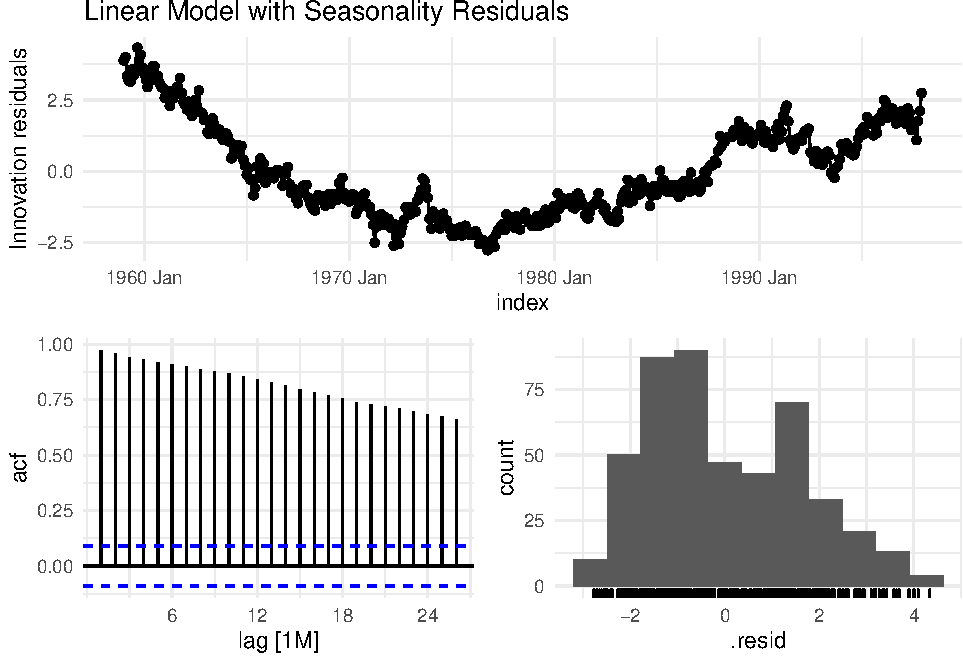
\includegraphics{co2_1997_Qian_files/figure-latex/seasonalized model residulas-1.pdf}

The residuals for this model, however, result in lags that are all
autocorrelated and a residual plot that forms a parabolic pattern, which
is evidence against the hypothesis that a linear model can appropriately
fit the data. A polynomial model may therefore be a more sensible option
in order to capture the non-linearities in the data, so we then fit the
following quadratic model:

\begin{equation}
\label{eq:one}
\text{CO}_{2} = \beta_0 + \beta_1 t + \beta_2 t^2
\end{equation}

Estimating the parameters as follows,

\begin{Shaded}
\begin{Highlighting}[]
\NormalTok{co2\_quadratic }\OtherTok{\textless{}{-}}\NormalTok{ ts\_co2 }\SpecialCharTok{\%\textgreater{}\%} 
    \FunctionTok{model}\NormalTok{(}\FunctionTok{TSLM}\NormalTok{(value }\SpecialCharTok{\textasciitilde{}} \FunctionTok{trend}\NormalTok{() }\SpecialCharTok{+} \FunctionTok{I}\NormalTok{(}\FunctionTok{trend}\NormalTok{()}\SpecialCharTok{\^{}}\DecValTok{2}\NormalTok{))) }\SpecialCharTok{\%\textgreater{}\%} 
    \FunctionTok{report}\NormalTok{()}
\end{Highlighting}
\end{Shaded}

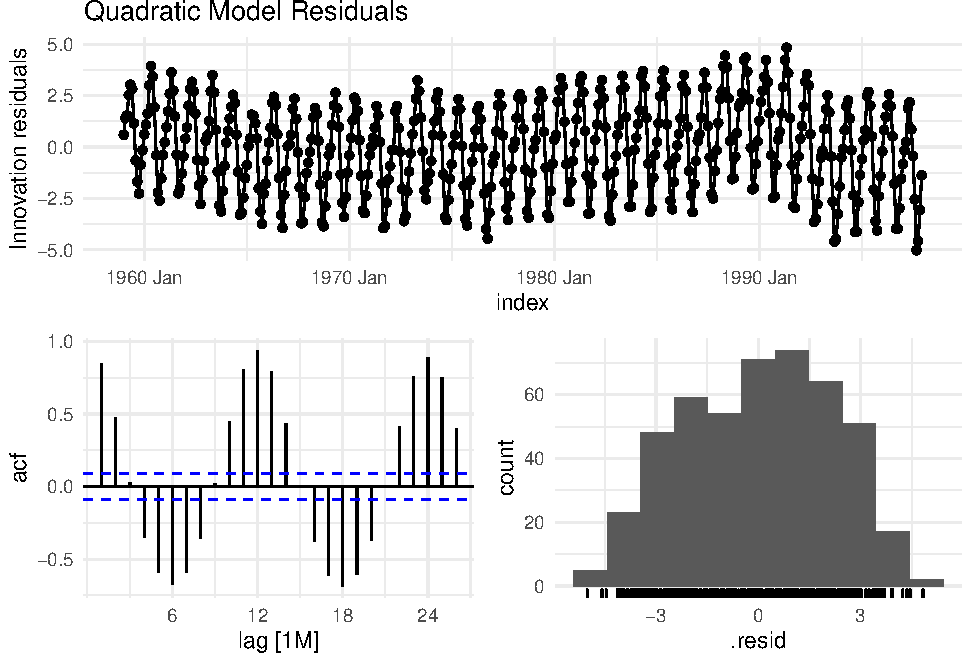
\includegraphics{co2_1997_Qian_files/figure-latex/Quad model residuals-1.pdf}

The result is a more white-noise-like residual plot, but with strong
seasonality still being showcased in the ACF plot. We can now attempt to
rectify for the seasonality once more with the addition of a seasonal
dummy variable,

\begin{Shaded}
\begin{Highlighting}[]
\NormalTok{co2\_quadratic\_season }\OtherTok{\textless{}{-}}\NormalTok{ ts\_co2 }\SpecialCharTok{\%\textgreater{}\%} 
    \FunctionTok{model}\NormalTok{(}\FunctionTok{TSLM}\NormalTok{(value }\SpecialCharTok{\textasciitilde{}} \FunctionTok{trend}\NormalTok{() }\SpecialCharTok{+} \FunctionTok{I}\NormalTok{(}\FunctionTok{trend}\NormalTok{()}\SpecialCharTok{\^{}}\DecValTok{2}\NormalTok{) }\SpecialCharTok{+} \FunctionTok{season}\NormalTok{())) }\SpecialCharTok{\%\textgreater{}\%} 
    \FunctionTok{report}\NormalTok{()}
\end{Highlighting}
\end{Shaded}

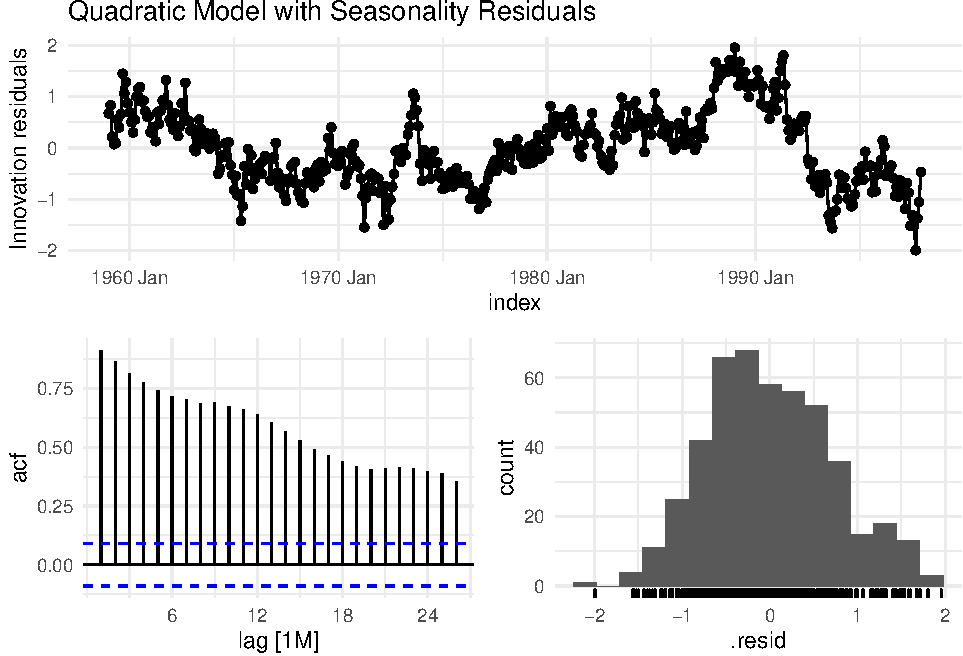
\includegraphics{co2_1997_Qian_files/figure-latex/Quad model with seasonality residuals-1.pdf}

but despite the addition of the seasonal term, a subtle seasonal pattern
can still be observed in the ACF, along with all significant lags and
strong autocorrelation in the ACF.

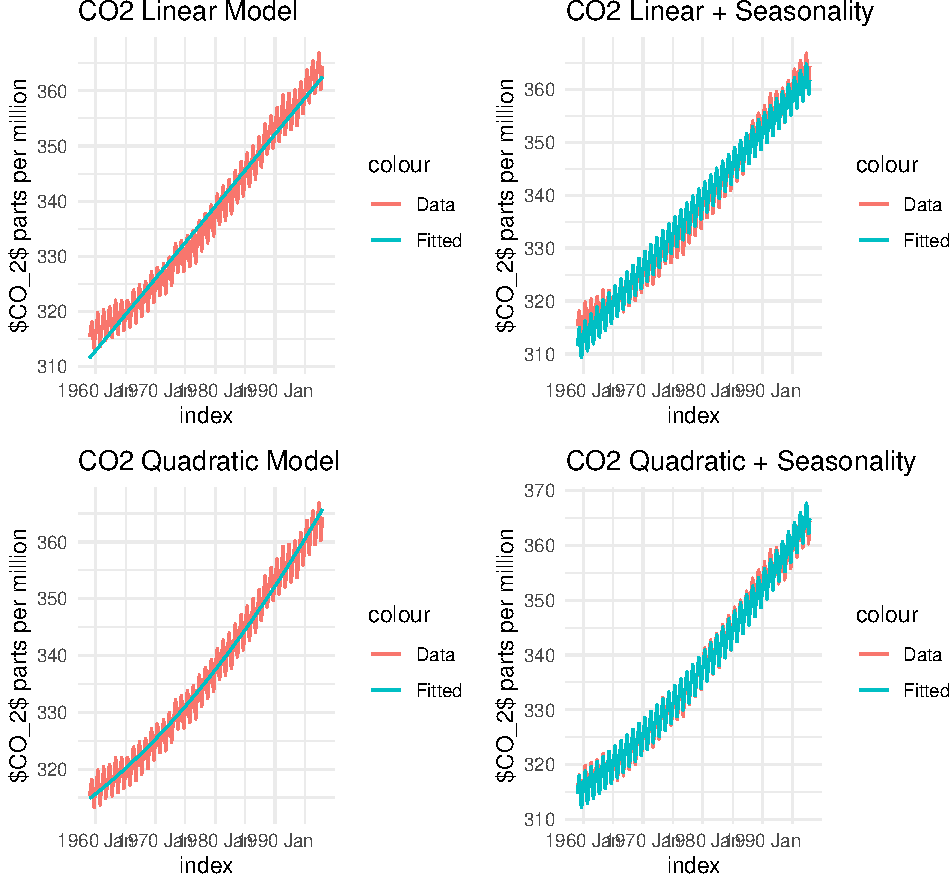
\includegraphics{co2_1997_Qian_files/figure-latex/unnamed-chunk-1-1.pdf}

From the fitted value plots, we can see that the simple linear and
quadratic models capture the trend quite well, but fail to capture the
seasonal fluctuations present in the data, although it's important to
note that the quadratic model was slightly more successful at this than
the linear model. The linear model corrected for seasonality attempts to
better capture the seasonal effect and does much better job at doing so,
but it underestimates the observed data. In the end, our final quadratic
model with the additional seasonal dummy variable seems to do a good job
capturing both trend and seasonal movement in the data,

\begin{longtable}[]{@{}rrrrrl@{}}
\toprule
adj\_r\_squared & CV & AIC & AICc & BIC & name \\
\midrule
\endhead
0.998 & 0.541 & -286 & -285 & -224 & Quadratic + Seasonality \\
0.988 & 2.759 & 476 & 477 & 534 & Linear + Seasonality \\
0.979 & 4.794 & 735 & 735 & 752 & Quadratic \\
0.969 & 6.889 & 905 & 905 & 917 & Linear \\
\bottomrule
\end{longtable}

and a quick calculation of the AIC, AICc, and BIC of all tested models
confirms this theory as it has the lowest value for all aforementioned
information criterion.

\begin{longtable}[]{@{}lrr@{}}
\toprule
.model & lb\_stat & lb\_pvalue \\
\midrule
\endhead
TSLM(value \textasciitilde{} trend()) & 2974 & 0 \\
TSLM(value \textasciitilde{} trend() + season()) & 8011 & 0 \\
TSLM(value \textasciitilde{} trend() + I(trend()\^{}2)) & 3838 & 0 \\
TSLM(value \textasciitilde{} trend() + I(trend()\^{}2) + season()) &
4441 & 0 \\
\bottomrule
\end{longtable}

From the Ljung Box test results, the statistic for all models are high
and the p-value are small, we reject the null hypothesis of no
autocorrelation. We can conclude that the residuals are auto-correlated.

We then evaluate a logarithmic transformation of the data in order to
gauge whether it would be a worthwhile transformation to consider in
trying to improve the fit of our models.

\begin{Shaded}
\begin{Highlighting}[]
\NormalTok{ts\_log\_co2 }\OtherTok{\textless{}{-}}\NormalTok{ ts\_co2 }\SpecialCharTok{\%\textgreater{}\%} 
      \FunctionTok{mutate}\NormalTok{(}\AttributeTok{log\_co2 =} \FunctionTok{log}\NormalTok{(value))}
\FunctionTok{head}\NormalTok{(ts\_log\_co2) }\SpecialCharTok{\%\textgreater{}\%}\NormalTok{ knitr}\SpecialCharTok{::}\FunctionTok{kable}\NormalTok{()}
\end{Highlighting}
\end{Shaded}

\begin{longtable}[]{@{}lrr@{}}
\toprule
index & value & log\_co2 \\
\midrule
\endhead
1959 Jan & 315 & 5.75 \\
1959 Feb & 316 & 5.76 \\
1959 Mar & 316 & 5.76 \\
1959 Apr & 318 & 5.76 \\
1959 May & 318 & 5.76 \\
1959 Jun & 318 & 5.76 \\
\bottomrule
\end{longtable}

Then new log-transformed data is now used to change the response
variable of \(CO_2\) for the same four previous models,

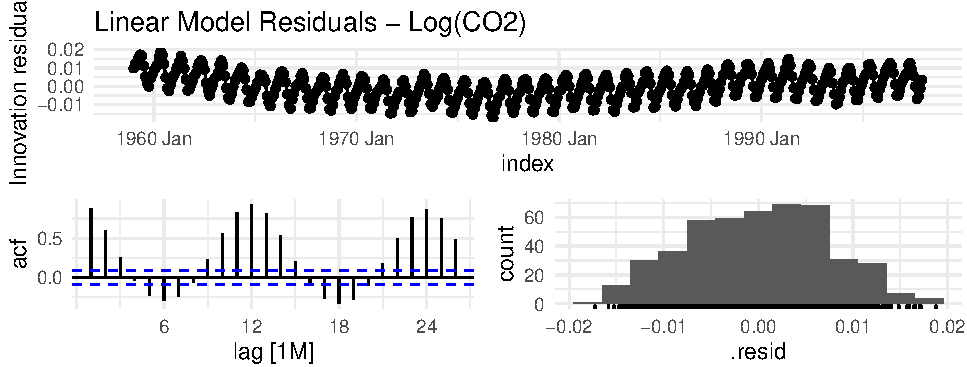
\includegraphics{co2_1997_Qian_files/figure-latex/linear log models, -1.pdf}

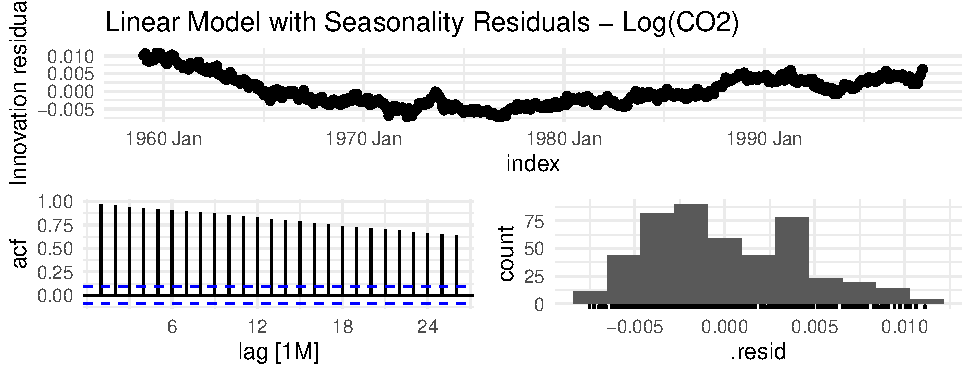
\includegraphics{co2_1997_Qian_files/figure-latex/linear seasonal log transform-1.pdf}

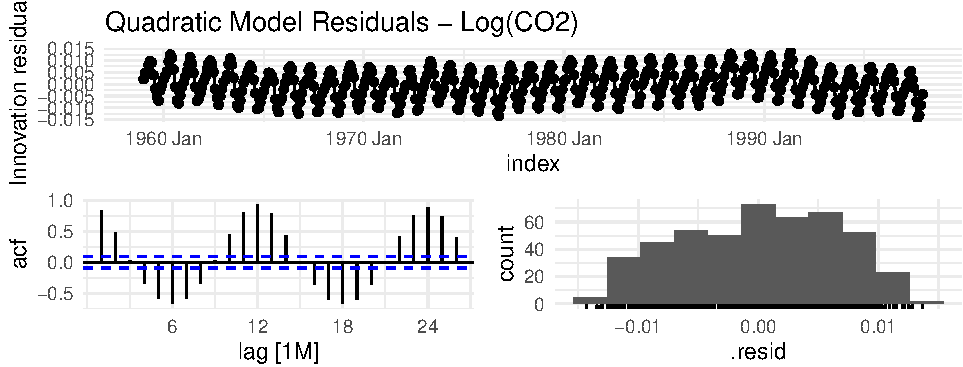
\includegraphics{co2_1997_Qian_files/figure-latex/quad log transform-1.pdf}

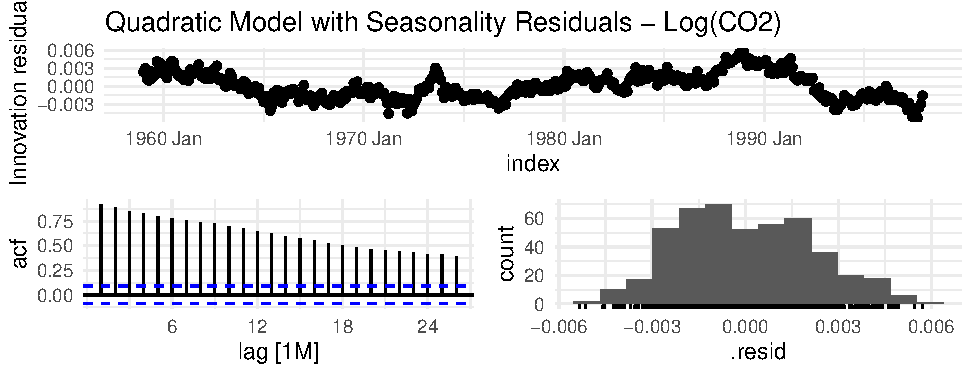
\includegraphics{co2_1997_Qian_files/figure-latex/quad seasonal log transform-1.pdf}

and no significant change can be observed in the residuals of the
models. This is to be expected, however, as the exploratory data
analysis above did not show a clear exponential trend in the \(CO_2\)
data that would need to be smoothed and correct with a logarithmic
transformation, and the variance did not appear to increase or decrease
over time. Therefore, a logarithmic transformation is not exactly
necessary for modeling the \(CO_2\) data.

We further put our best quadratic with seasonality model to the test by
generating forecasts to the year 2020, and graphing the results:

\begin{Shaded}
\begin{Highlighting}[]
\CommentTok{\# Create a forecast object based on the model and forecast to the year 2020}
\FunctionTok{save}\NormalTok{(co2\_quadratic\_season, }\AttributeTok{file=}\StringTok{\textquotesingle{}1997\_quad\_seasonal\_modelfit.RData\textquotesingle{}}\NormalTok{)}
\NormalTok{quad.forecast }\OtherTok{\textless{}{-}}\NormalTok{ fabletools}\SpecialCharTok{::}\FunctionTok{forecast}\NormalTok{(co2\_quadratic\_season, }\AttributeTok{h =} \StringTok{"23 years"}\NormalTok{)}
\CommentTok{\# Forecast + previous data graph}
\NormalTok{forecast.graph }\OtherTok{\textless{}{-}}\NormalTok{ quad.forecast }\SpecialCharTok{\%\textgreater{}\%} \FunctionTok{autoplot}\NormalTok{(ts\_co2) }\SpecialCharTok{+} \FunctionTok{labs}\NormalTok{(}\AttributeTok{title=}\StringTok{"Linear model forecast 1997{-}2020"}\NormalTok{, }\AttributeTok{x=}\ConstantTok{NULL}\NormalTok{, }\AttributeTok{y=}\StringTok{"Monthly mean CO2 ppm"}\NormalTok{)}
\NormalTok{forecast.graph}
\end{Highlighting}
\end{Shaded}

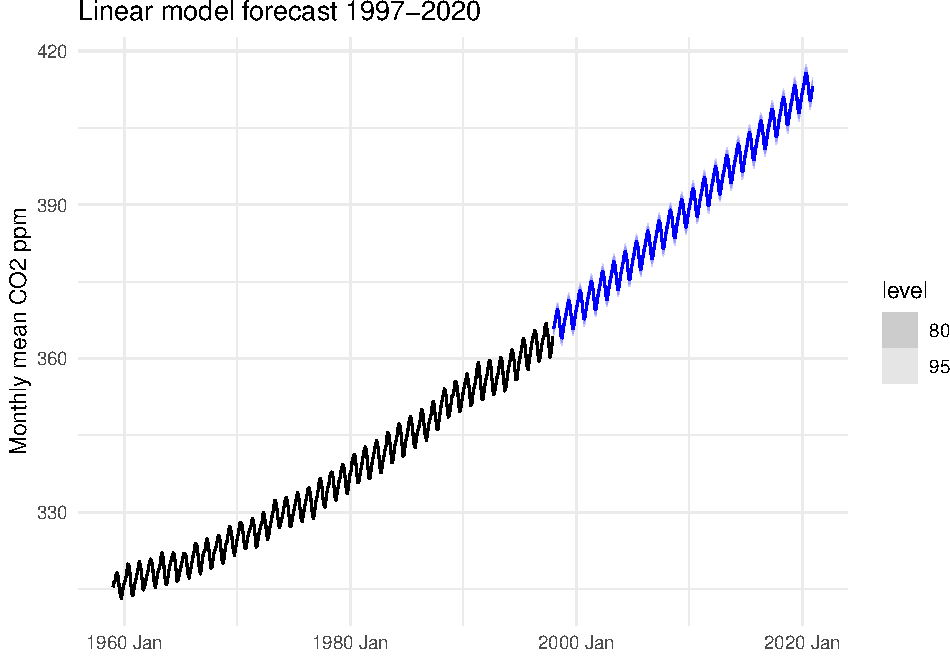
\includegraphics{co2_1997_Qian_files/figure-latex/Forecast till 2020-1.pdf}

Although the forecast seems to follow along the same patterns as past
\(CO_2\) data, there's strong evidence from the high autocorrelation
observed in the ACF of the model residuals and the lack of observed
white noise residuals that this model does not perfectly fit our model.
This therefore motivates exploring an ARIMA model and checking the first
difference.

\hypertarget{arima-models}{%
\subsection{ARIMA Models}\label{arima-models}}

We begin by first differencing the \(CO_2\) data:

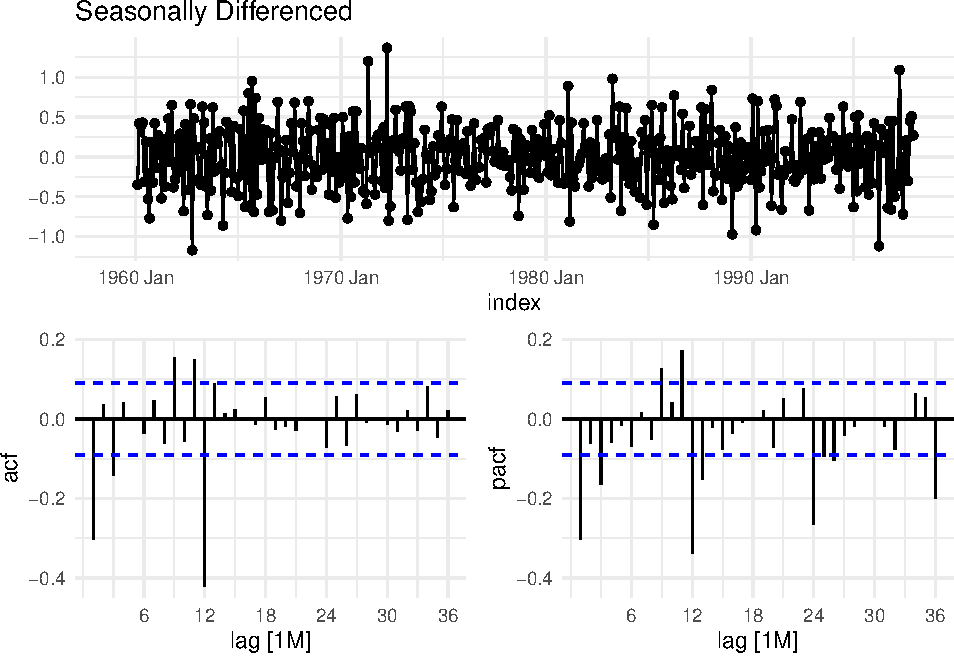
\includegraphics{co2_1997_Qian_files/figure-latex/unnamed-chunk-2-1.pdf}

From the EDA, we found the \(CO_2\) time series had obvious trend and
seasonality. Based on the time series plot of the first difference, we
now observe that the data's first difference may be stationary, and from
the ACF plot, we see seasonal fluctuations every 12 lags (months). A
Phillips-Perron and Augmented Dickey-Fuller test can then be run to test
the alternate hypothesis that the time series is stationary, as opposed
to the null hypothesis that it is explosive, or non stationary.

\begin{Shaded}
\begin{Highlighting}[]
\FunctionTok{PP.test}\NormalTok{(co2\_diff)}
\end{Highlighting}
\end{Shaded}

\begin{verbatim}
## 
##  Phillips-Perron Unit Root Test
## 
## data:  co2_diff
## Dickey-Fuller = -9, Truncation lag parameter = 5, p-value = 0.01
\end{verbatim}

\begin{Shaded}
\begin{Highlighting}[]
\FunctionTok{adf.test}\NormalTok{(co2\_diff, }\AttributeTok{alternative =} \StringTok{"stationary"}\NormalTok{)}
\end{Highlighting}
\end{Shaded}

\begin{verbatim}
## 
##  Augmented Dickey-Fuller Test
## 
## data:  co2_diff
## Dickey-Fuller = -30, Lag order = 7, p-value = 0.01
## alternative hypothesis: stationary
\end{verbatim}

Both the Phillips Perron and Augmented Dickey Fuller (ADF) tests show a
p-value that is less than \(0.05\), therefore providing strong evidence
for us to reject the null hypothesis that this time series is non
stationary. Thus, the time series with the first difference is
stationary and we can start to build the model with 1 difference.

\begin{Shaded}
\begin{Highlighting}[]
\NormalTok{fit }\SpecialCharTok{\%\textgreater{}\%}
  \FunctionTok{report}\NormalTok{() }\SpecialCharTok{\%\textgreater{}\%} \FunctionTok{arrange}\NormalTok{(AIC) }\SpecialCharTok{\%\textgreater{}\%} 
  \FunctionTok{select}\NormalTok{(}\SpecialCharTok{{-}}\NormalTok{ar\_roots, }\SpecialCharTok{{-}}\NormalTok{ma\_roots) }\SpecialCharTok{\%\textgreater{}\%}\NormalTok{ knitr}\SpecialCharTok{::}\FunctionTok{kable}\NormalTok{()}
\end{Highlighting}
\end{Shaded}

\begin{verbatim}
## Warning in report.mdl_df(.): Model reporting is only supported for individual
## models, so a glance will be shown. To see the report for a specific model, use
## `select()` and `filter()` to identify a single model.
\end{verbatim}

\begin{longtable}[]{@{}lrrrrr@{}}
\toprule
.model & sigma2 & log\_lik & AIC & AICc & BIC \\
\midrule
\endhead
auto & 0.085 & -83.4 & 177 & 177 & 197 \\
arima012011 & 0.086 & -85.5 & 179 & 179 & 196 \\
arima111112 & 0.086 & -84.4 & 181 & 181 & 205 \\
arima210011 & 0.087 & -87.7 & 183 & 184 & 200 \\
arima214000 & 0.290 & -373.3 & 763 & 763 & 796 \\
arima111000 & 0.631 & -554.5 & 1115 & 1115 & 1128 \\
arima121000 & 0.785 & -603.7 & 1213 & 1213 & 1226 \\
\bottomrule
\end{longtable}

\begin{Shaded}
\begin{Highlighting}[]
\NormalTok{fit}\SpecialCharTok{$}\NormalTok{auto[[}\DecValTok{1}\NormalTok{]]}\SpecialCharTok{$}\NormalTok{fit}\SpecialCharTok{$}\NormalTok{spec }\SpecialCharTok{\%\textgreater{}\%}\NormalTok{ knitr}\SpecialCharTok{::}\FunctionTok{kable}\NormalTok{()}
\end{Highlighting}
\end{Shaded}

\begin{longtable}[]{@{}rrrrrrlr@{}}
\toprule
p & d & q & P & D & Q & constant & period \\
\midrule
\endhead
0 & 1 & 3 & 0 & 1 & 1 & FALSE & 12 \\
\bottomrule
\end{longtable}

\begin{Shaded}
\begin{Highlighting}[]
\NormalTok{fit}\SpecialCharTok{$}\NormalTok{auto[[}\DecValTok{1}\NormalTok{]]}\SpecialCharTok{$}\NormalTok{fit}\SpecialCharTok{$}\NormalTok{model}
\end{Highlighting}
\end{Shaded}

\begin{verbatim}
## 
## Call:
## .f(x = ..1, order = ..2, seasonal = ..3, xreg = ..4, include.mean = FALSE, fixed = ..7, 
##     method = ..5)
## 
## Coefficients:
##          ma1     ma2     ma3    sma1
##       -0.339  -0.018  -0.097  -0.854
## s.e.   0.048   0.050   0.047   0.026
## 
## sigma^2 estimated as 0.0852:  log likelihood = -83.4,  aic = 177
\end{verbatim}

After fitting numerous ARIMA models with varying specifications and
running the auto model as well, we find that based on the AIC, AICc
scores displayed in the table above, the auto model found to be
ARIMA(0,1,3),(0,1,1)(12) has the lowest scores and is therefore the best
fit model. When looking at the BIC scores, however, the lowest value was
found to be for the ARIMA(0,1,2),(0,1,1)(12) model. Since we are aiming
to complete more of a prediction task with our forecasting efforts
rather than an explanation task and that AIC is most optimal in
minimizing the mean squared error of predictions, we choose to use
AIC/AICc as our main information criteria. The best fit model is
therefore ARIMA(0,1,3),(0,1,1)(12), which we fit next:

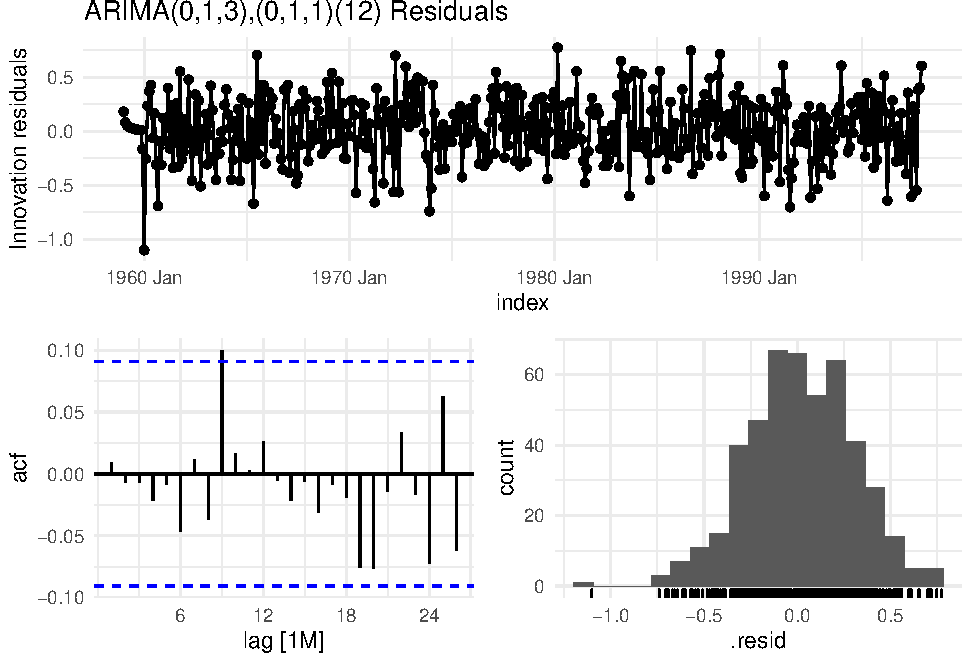
\includegraphics{co2_1997_Qian_files/figure-latex/Best ARIMA model residual-1.pdf}

The flat mean of the residuals at 0, the roughly normally distributed
residual counts, and the minimally autocorrelated/significant lags in
the ACF are all strong evidence that we have white noise residuals and
that the ARIMA(0,1,3),(0,1,1)(12) model fits the \(CO_2\) model well.

\begin{Shaded}
\begin{Highlighting}[]
\FunctionTok{augment}\NormalTok{(arima013011) }\SpecialCharTok{\%\textgreater{}\%}
    \FunctionTok{features}\NormalTok{(.resid, ljung\_box, }\AttributeTok{lag =} \DecValTok{10}\NormalTok{, }\AttributeTok{dof =} \DecValTok{0}\NormalTok{)}
\end{Highlighting}
\end{Shaded}

\begin{verbatim}
## # A tibble: 1 x 3
##   .model      lb_stat lb_pvalue
##   <chr>         <dbl>     <dbl>
## 1 arima013011    7.01     0.724
\end{verbatim}

From the Ljung Box test, we got a large p-value that failed to reject
the null hypothesis, further supporting that our best model's residuals
are randomly distributed, thus making it a good model fit. Generating
forecast to the year 2022 with the new ARIMA model shows that the model
follows the pattern of past data fairly well.

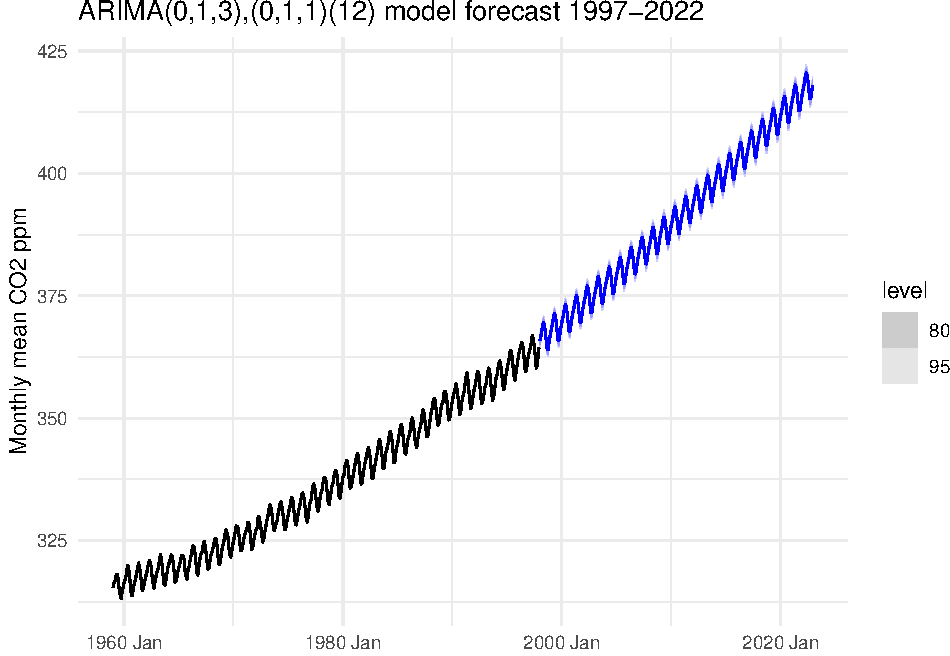
\includegraphics{co2_1997_Qian_files/figure-latex/ARIMA Forecast till 2020-1.pdf}

\hypertarget{forecasts}{%
\subsection{Forecasts}\label{forecasts}}

Further forecasts can be generated to the year 2100 to test our model
and make predictions about the future. We see the performance within
80\% and 95\% confidence intervals below, and the times the 420 and 500
ppm thersholds are crossed within the forecasts.

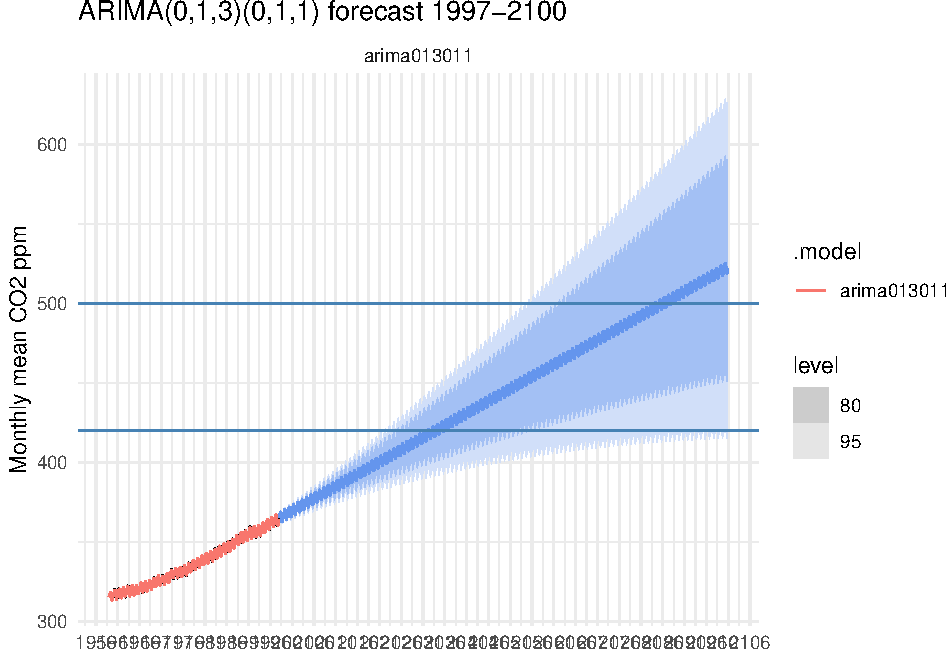
\includegraphics{co2_1997_Qian_files/figure-latex/ARIMA forecast plot-1.pdf}

\begin{longtable}[]{@{}
  >{\raggedleft\arraybackslash}p{(\columnwidth - 12\tabcolsep) * \real{0.1000}}
  >{\raggedright\arraybackslash}p{(\columnwidth - 12\tabcolsep) * \real{0.1286}}
  >{\raggedleft\arraybackslash}p{(\columnwidth - 12\tabcolsep) * \real{0.0857}}
  >{\raggedleft\arraybackslash}p{(\columnwidth - 12\tabcolsep) * \real{0.1714}}
  >{\raggedleft\arraybackslash}p{(\columnwidth - 12\tabcolsep) * \real{0.1714}}
  >{\raggedleft\arraybackslash}p{(\columnwidth - 12\tabcolsep) * \real{0.1714}}
  >{\raggedleft\arraybackslash}p{(\columnwidth - 12\tabcolsep) * \real{0.1714}}@{}}
\toprule
\begin{minipage}[b]{\linewidth}\raggedleft
target
\end{minipage} & \begin{minipage}[b]{\linewidth}\raggedright
index
\end{minipage} & \begin{minipage}[b]{\linewidth}\raggedleft
.mean
\end{minipage} & \begin{minipage}[b]{\linewidth}\raggedleft
ci.80.lower
\end{minipage} & \begin{minipage}[b]{\linewidth}\raggedleft
ci.80.upper
\end{minipage} & \begin{minipage}[b]{\linewidth}\raggedleft
ci.95.lower
\end{minipage} & \begin{minipage}[b]{\linewidth}\raggedleft
ci.95.upper
\end{minipage} \\
\midrule
\endhead
420 & 2032 Apr & 420 & 405 & 436 & 397 & 444 \\
420 & 2036 Sep & 421 & 403 & 439 & 393 & 449 \\
500 & 2084 Apr & 500 & 447 & 553 & 419 & 582 \\
500 & 2088 Oct & 501 & 444 & 558 & 413 & 588 \\
\bottomrule
\end{longtable}

The forecasts for the year 2100 in particular can be seen below:

\begin{longtable}[]{@{}lrrrrr@{}}
\toprule
index & .mean & ci.80.lower & ci.80.upper & ci.95.lower & ci.95.upper \\
\midrule
\endhead
2100 Jan & 522 & 454 & 589 & 419 & 625 \\
2100 Feb & 522 & 455 & 590 & 419 & 626 \\
2100 Mar & 523 & 456 & 591 & 420 & 627 \\
2100 Apr & 525 & 457 & 592 & 421 & 628 \\
2100 May & 525 & 458 & 593 & 422 & 629 \\
2100 Jun & 525 & 457 & 592 & 421 & 628 \\
2100 Jul & 523 & 455 & 591 & 419 & 627 \\
2100 Aug & 521 & 453 & 589 & 417 & 625 \\
2100 Sep & 519 & 451 & 587 & 415 & 623 \\
2100 Oct & 519 & 451 & 587 & 415 & 623 \\
2100 Nov & 521 & 453 & 589 & 416 & 625 \\
2100 Dec & 522 & 454 & 590 & 418 & 627 \\
\bottomrule
\end{longtable}

Although it follows the pattern of past data well, it's difficult to say
if these are accurate predictions for the future, but if the current
trends persist through to the year 2100, then these predictions may not
be far off from the true values we will observe in \(CO_2\) then.

\hypertarget{conclusions}{%
\section{Conclusions}\label{conclusions}}

From the modeling and analysis on atmospheric \(CO_{2}\) data from 1959
to 1997, we achieved our goals to answer the initial questions. Firstly,
we observed and demonstrated that CO2 concentrations in the Earth's
atmosphere have been increasing steadily from 1959 to 1997 and will keep
increasing based on both the quadratic model and ARIMA forecast results.
Secondly, both linear model and ARIMA with seasonality have better
performance than models that didn't considering the seasonality.
Finally, the quadratic model with seasonality and
ARIMA(0,1,3),(0,1,1)(12) model fit \(CO_{2}\) data well, but there's
strong evidence that quadratic model has the high autocorrelation
observed in the ACF of the model residuals. Therefore, the most
plausible model that we estimate is ARIMA(0,1,3),(0,1,1)(12) model and
we can use this model to forecast the atmospheric \(CO_{2}\) changing.

\bibliographystyle{aea}
\bibliography{references}

\appendix
\section{Appendix: Model Robustness}


\end{document}
